\documentclass[12pt,a4paper,twoside,openany]{book}
\usepackage[]{graphicx}\usepackage[]{color}
%% maxwidth is the original width if it is less than linewidth
%% otherwise use linewidth (to make sure the graphics do not exceed the margin)
\makeatletter
\def\maxwidth{ %
  \ifdim\Gin@nat@width>\linewidth
    \linewidth
  \else
    \Gin@nat@width
  \fi
}
\makeatother

\definecolor{fgcolor}{rgb}{0.345, 0.345, 0.345}
\newcommand{\hlnum}[1]{\textcolor[rgb]{0.686,0.059,0.569}{#1}}%
\newcommand{\hlstr}[1]{\textcolor[rgb]{0.192,0.494,0.8}{#1}}%
\newcommand{\hlcom}[1]{\textcolor[rgb]{0.678,0.584,0.686}{\textit{#1}}}%
\newcommand{\hlopt}[1]{\textcolor[rgb]{0,0,0}{#1}}%
\newcommand{\hlstd}[1]{\textcolor[rgb]{0.345,0.345,0.345}{#1}}%
\newcommand{\hlkwa}[1]{\textcolor[rgb]{0.161,0.373,0.58}{\textbf{#1}}}%
\newcommand{\hlkwb}[1]{\textcolor[rgb]{0.69,0.353,0.396}{#1}}%
\newcommand{\hlkwc}[1]{\textcolor[rgb]{0.333,0.667,0.333}{#1}}%
\newcommand{\hlkwd}[1]{\textcolor[rgb]{0.737,0.353,0.396}{\textbf{#1}}}%
\let\hlipl\hlkwb

\usepackage{framed}
\makeatletter
\newenvironment{kframe}{%
 \def\at@end@of@kframe{}%
 \ifinner\ifhmode%
  \def\at@end@of@kframe{\end{minipage}}%
  \begin{minipage}{\columnwidth}%
 \fi\fi%
 \def\FrameCommand##1{\hskip\@totalleftmargin \hskip-\fboxsep
 \colorbox{shadecolor}{##1}\hskip-\fboxsep
     % There is no \\@totalrightmargin, so:
     \hskip-\linewidth \hskip-\@totalleftmargin \hskip\columnwidth}%
 \MakeFramed {\advance\hsize-\width
   \@totalleftmargin\z@ \linewidth\hsize
   \@setminipage}}%
 {\par\unskip\endMakeFramed%
 \at@end@of@kframe}
\makeatother

\definecolor{shadecolor}{rgb}{.97, .97, .97}
\definecolor{messagecolor}{rgb}{0, 0, 0}
\definecolor{warningcolor}{rgb}{1, 0, 1}
\definecolor{errorcolor}{rgb}{1, 0, 0}
\newenvironment{knitrout}{}{} % an empty environment to be redefined in TeX

\usepackage{alltt}
\newcommand{\SweaveOpts}[1]{}  % do not interfere with LaTeX
\newcommand{\SweaveInput}[1]{} % because they are not real TeX commands
\newcommand{\Sexpr}[1]{}       % will only be parsed by R


\usepackage[margin=48pt]{geometry}
\usepackage{amsthm}
\usepackage{amssymb}
\usepackage{amsmath}
\usepackage{parskip}
\usepackage{graphicx}
\usepackage{enumerate}
\usepackage{subcaption}
\usepackage[table]{xcolor}

\usepackage{float}
\floatstyle{boxed} 
\restylefloat{figure}

\usepackage{setspace}
\doublespacing

\usepackage{listings}
\usepackage{bm}
\usepackage{natbib}%citation purposes


\newcommand{\BI}[1]{\textit{\textbf{#1}}}
\newcommand{\me}{\mathrm{e}}




\begin{document}
% This is the text for chapter 3 of the report



\chapter{Application}
Most of application in ERGM Count has been focusing on social network analysis. 
Whether it is ... and ... 

Here we will fit English Premier League(EPL) data to ERGM COunt.
EPL is the top tier of footbal competition in England.
It is regarded as the world most watched sports league in the world. 

At the first glance, it may not be seem that EPL exhibit a graph representation. We will try to justify the fitting of ERGM Count in the next section.  

\section{Justification ERGM Count Fitting}

In EPL there are 20 teams which represent the nodes of the graph. There will be football matches wehre 2 teams will be playing aginst one another. 
Within 90 minutes period, each team are supposed to score as many goals as possible to the opponent.
At the end of the match the team with the highest accumulated goals will win the match. 
We can then define $y_{ij}$ as the total number of goals scored from team $i$ to team $j$.
The opposing edge $y_{ji}$ will then represent the number of goals from team $i$ to team $j$ in the same match. 
The game may end up in draw if both of the team have equal goals.
On halfway of the league, each team has finished exactly one match against every other team. 
The graph is now complete such that, all the edges combination have probability to attain values other than 0. 
We can then fit ERGM Count to the EPL data.
One example of the graph that will be fitted is shown in Figure \ref{fig:EPL2015}

\begin{figure}[H]
\begin{knitrout}
\definecolor{shadecolor}{rgb}{0.969, 0.969, 0.969}\color{fgcolor}

{\centering \includegraphics[width=\maxwidth]{figure/unnamed-chunk-1-1} 

}



\end{knitrout}
\caption [Graph Representation of a Football League]{This is the graph representation of the dataset used. The circles denote the 20 teams that are participating. The participating teams vary annually. The size of the circles corresponds to the average market value of the players in the team. The bigger the circle, the average price of the players is higher. The arrow represents the goal scored by the team it orginates from, to the team pointed by the arrow head. The green hue indicates the scoring team is playing at home stadium. Whereas the red hue shows the goal scored in opponent stadium. The intensity of the color represents the total goal scored. The higher intensity of the color, the more goals were scored.}
\label{fig: EPL}
\end{figure}


%This is for the igraph figure


\begin{figure}[H] % "[t!]" placement specifier just for this example

\hspace*{\fill}
\begin{subfigure}{0.40\textwidth}
\begin{knitrout}
\definecolor{shadecolor}{rgb}{0.969, 0.969, 0.969}\color{fgcolor}

{\centering 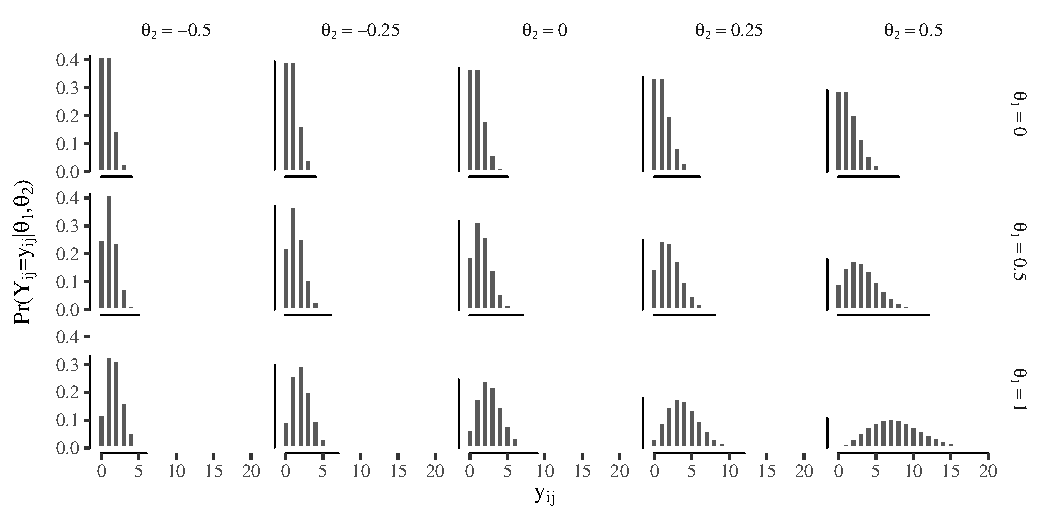
\includegraphics[width=\maxwidth]{figure/unnamed-chunk-3-1} 

}



\end{knitrout}
\caption{EPL 2013-2014, 1st Half}
\end{subfigure}\hspace*{\fill}
\begin{subfigure}{0.40\textwidth}
\begin{knitrout}
\definecolor{shadecolor}{rgb}{0.969, 0.969, 0.969}\color{fgcolor}

{\centering 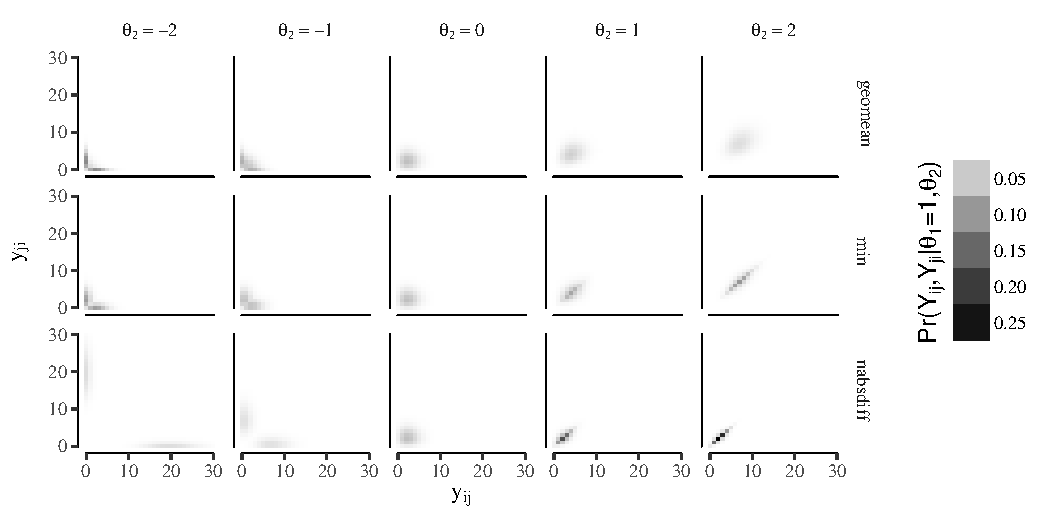
\includegraphics[width=\maxwidth]{figure/unnamed-chunk-4-1} 

}



\end{knitrout}
\caption{EPL 2013-2014, 2nd Half} 
\end{subfigure}
\hspace*{\fill}

\hspace*{\fill}
\begin{subfigure}{0.40\textwidth}
\begin{knitrout}
\definecolor{shadecolor}{rgb}{0.969, 0.969, 0.969}\color{fgcolor}

{\centering 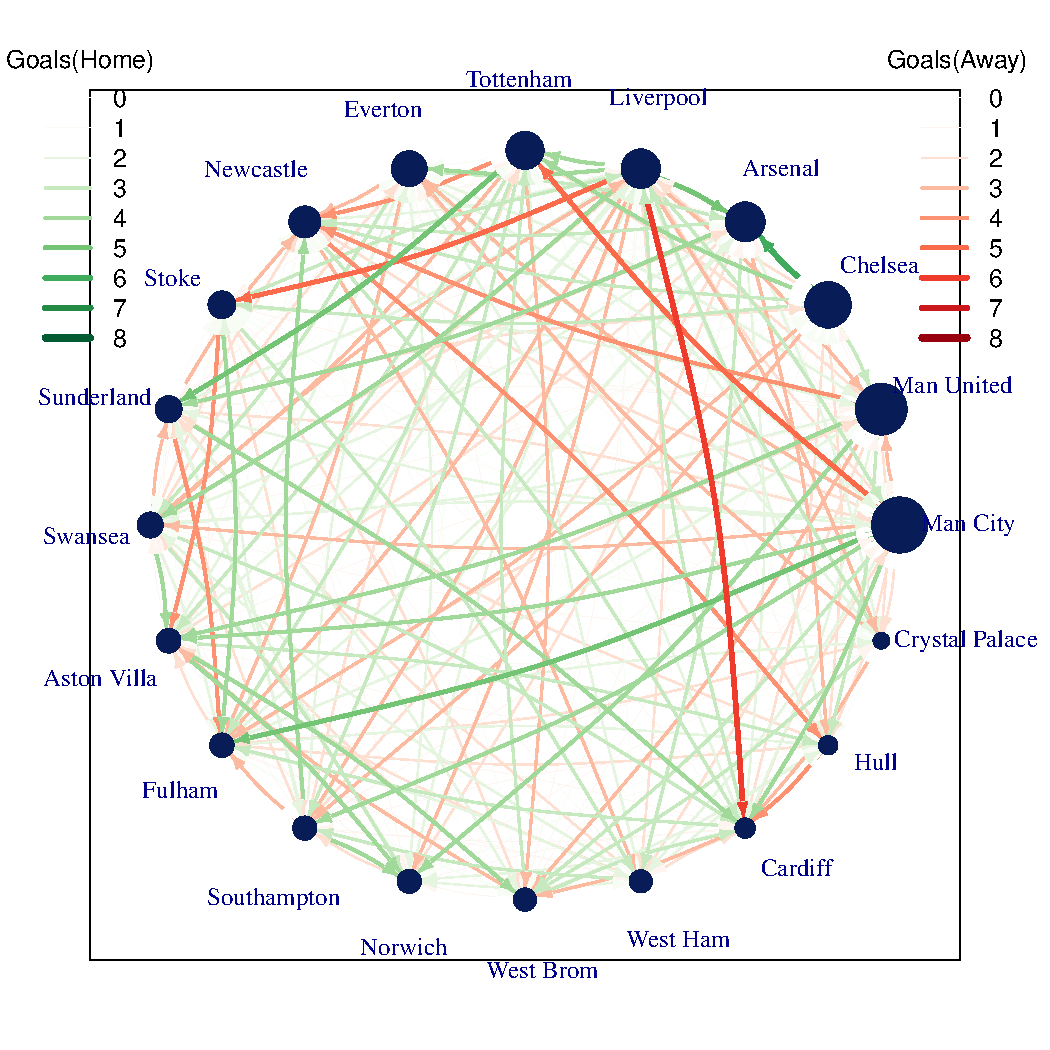
\includegraphics[width=\maxwidth]{figure/unnamed-chunk-5-1} 

}



\end{knitrout}
\caption{EPL 2014-2015, 1st Half}
\end{subfigure}\hspace*{\fill}
\begin{subfigure}{0.4\textwidth}
\begin{knitrout}
\definecolor{shadecolor}{rgb}{0.969, 0.969, 0.969}\color{fgcolor}

{\centering 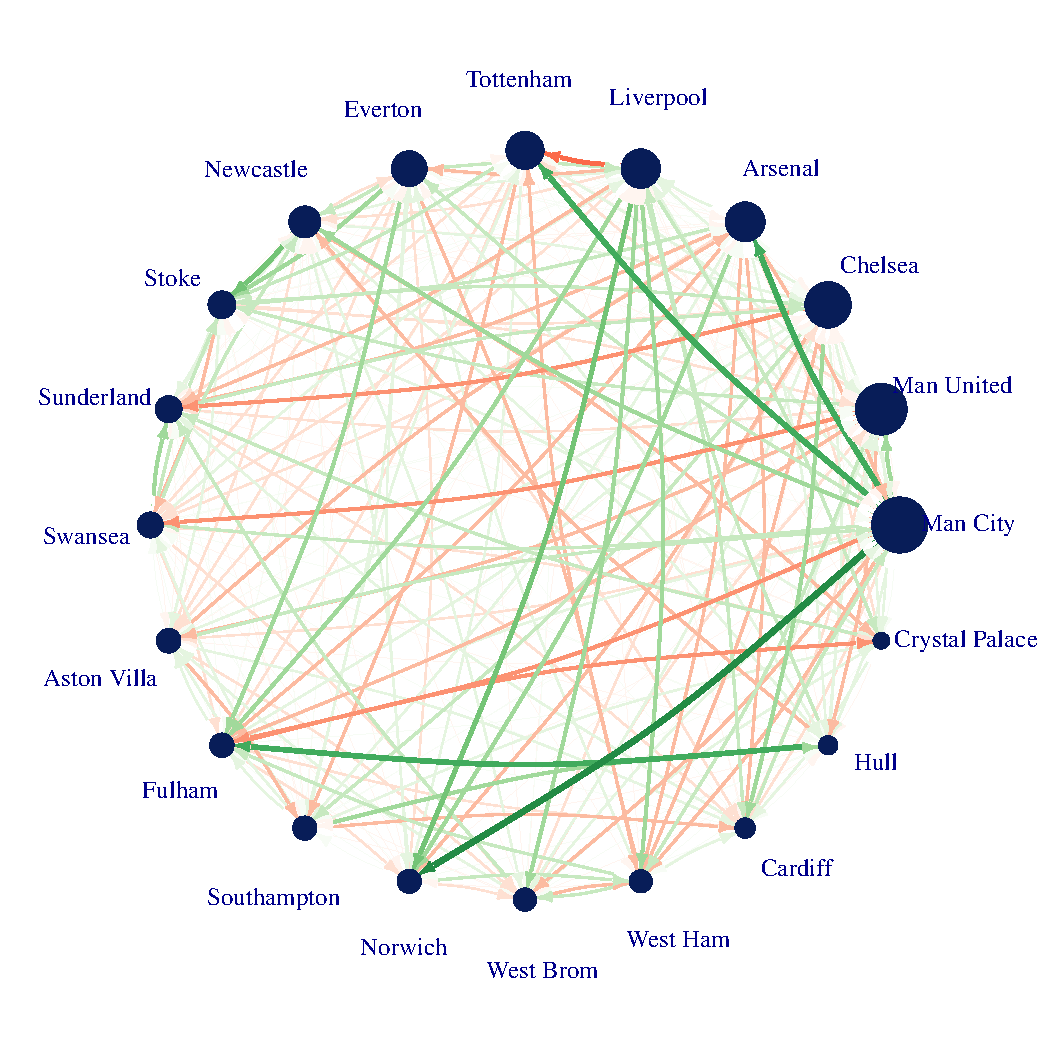
\includegraphics[width=\maxwidth]{figure/unnamed-chunk-6-1} 

}



\end{knitrout}
\caption{EPL 2014-2015, 2nd Half} 
\end{subfigure}
\hspace*{\fill}

\hspace*{\fill}
\begin{subfigure}{0.40\textwidth}
\begin{knitrout}
\definecolor{shadecolor}{rgb}{0.969, 0.969, 0.969}\color{fgcolor}

{\centering 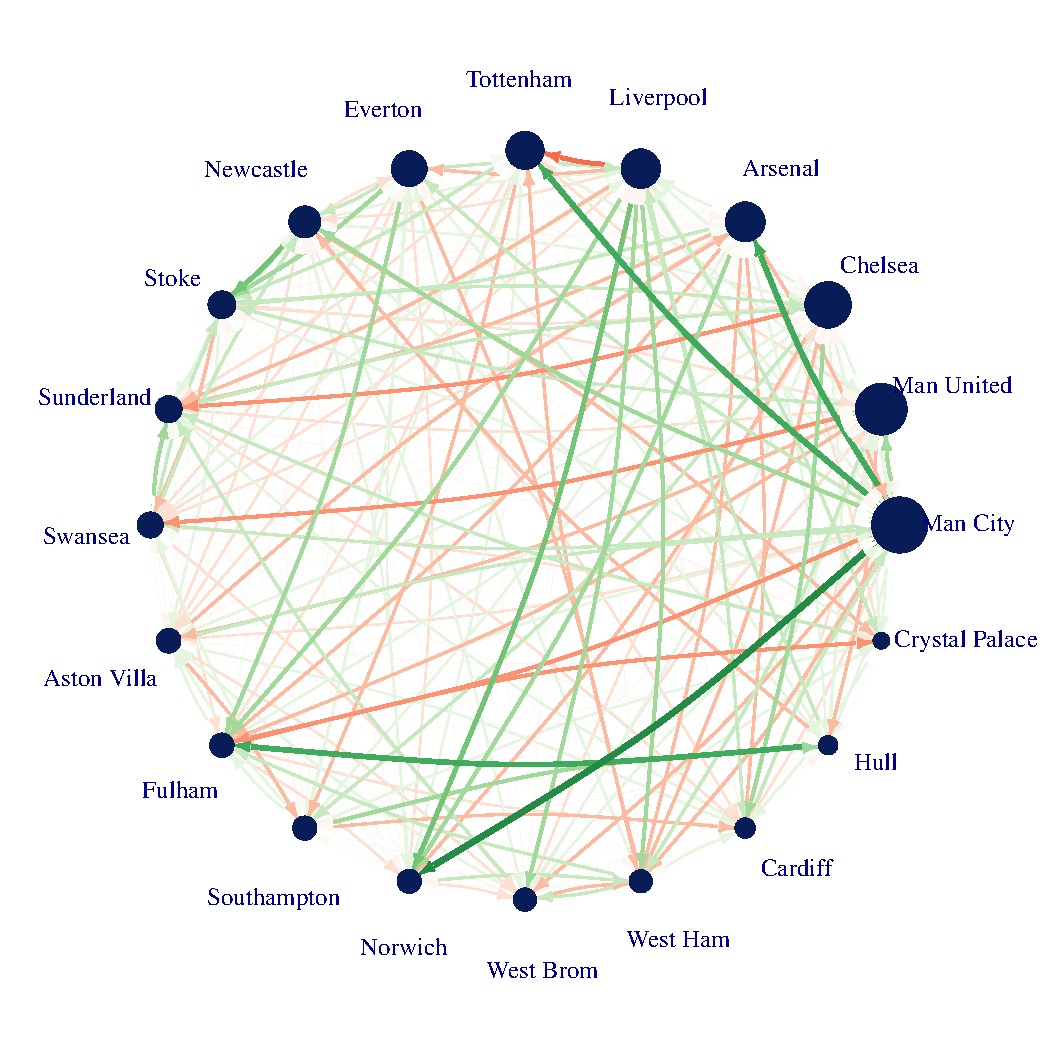
\includegraphics[width=\maxwidth]{figure/unnamed-chunk-7-1} 

}



\end{knitrout}
\caption{EPL 2015-2016, 1st Half}
\end{subfigure}\hspace*{\fill}
\begin{subfigure}{0.40\textwidth}
\begin{knitrout}
\definecolor{shadecolor}{rgb}{0.969, 0.969, 0.969}\color{fgcolor}

{\centering 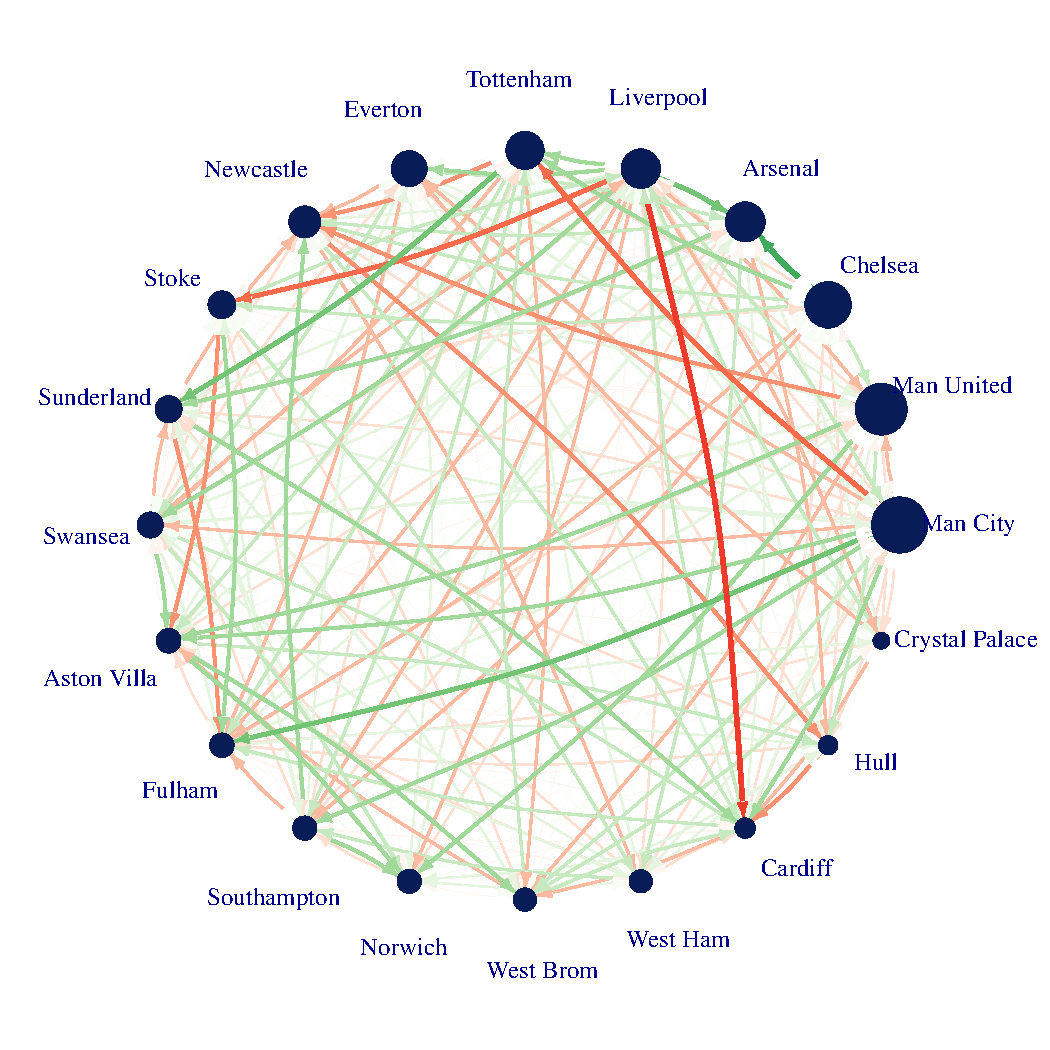
\includegraphics[width=\maxwidth]{figure/unnamed-chunk-8-1} 

}



\end{knitrout}
\caption{EPL 2015-2016, 2nd Half}
\end{subfigure}
\hspace*{\fill}
 
\caption [Graph Representation of a Football League]{This is the graph representation of the dataset used. The circles denote the 20 teams that are participating. The teams participating vary annually. Its size corresponds to the average market value of the players in the team. The bigger the circle, the average price of the players is higher. The arrow represents the goal scored by the team it orginates from, to the team pointed by the arrow head. The green hue indicates the scoring team is playing at home stadium. Whereas the red hue shows the goal scored in opponent stadium. The intensity of the color represents the total goals scored. The higher intensity of the color, the more goals were scored.} \label{fig:1}
\end{figure}

The interpretation of sufficient statistics will differs significantly from Krivistky's examples. 
First of all, it is unclear whether the goals scored can be modelled with Poisson or Geometric Distribution.
Maybe the \BI{nonzero} or \BI{CMP} distributions may also fit better. 
Here we are interested in finding the best shape of edge-wise distribution.
The notion behind the distribution is not of our interest.
For example, the goals may be well described by Geometric Distribution. 
However, the fact on Geometric Distribution represents the number of trials until the first success is not meaningful in this scenario.

Assuming Poisson Distribution is appropriate, we can further explore the exogenous covariates that may affect the mean. 
As mentioned in Figure \ref{fig:EPL2015}, one of the exogenous covariates is average market value of the players in the team attribute. 
This attribute will be explained further in Data Abstraction Section.
We will also consider whether 
There maybe other covariates that may provide a better fit.
However, as of now these 2 attributes are the only readily available data that is deemed to be appropriate.

Furthermore, we can assess the strength of the \BI{mutuality} of the network with ERGM Count.
Here \BI{mutuality} depicts the tendency for both teams in a match to score the same goals.
This seems to be unlikely as each team main goal is to win the match. 
Whereas the negative or \BI{anti-mutuality} can be interpreted as dominating effect.
When one of the team scores really high, the opposing tends to score low or none at all.
Anecdotal cases show such event may occur. 
We will investigate this effect further in Model Fitting and Analysis section.

The \BI{transitivity} attribute of the network is also interesting. 
If transitivity is found to be significant, when one team scores many goal to other team  

\section{More on The Data}
MOst of the data was retrieved from \textit{www.football-data.co.uk}.
The data files are downloadable csv files with consistent format for every different years.
These includes total goals scored by every team, from every football matches. 
The Home and Away attributes can also be abstracted easily from the files. 
There are many discrepancies in the name of the team with regards to the reality.
As a result, combining with other data source was found to be troublesome and laborious.

However, I managed to manually retrieve other attributes from \textit{www.transfermarkt.com}.
The attribute is the average market value of each player on that team during the particular competition period. 
The derivation of the market value of a player is not fully disclosed.
Users can express their opinion on the value itself.
Experts claim that there is high degree of correlation of the market value with actual sampled salary.
The market value has also been studied by ...

There are 6 complete graph that can be fit to each of different model. The data is summarised by the figure.

\section{Analysis on EPL based on ERGM Count}
\subsection{Analysis on Baseline Distribution}
We would like check whether 
\bibliography{my_bib}{}
\bibliographystyle{apalike}
\end{document}
